\documentclass{article}

\usepackage[table,xcdraw]{xcolor}
\usepackage{fancyhdr}
\usepackage{extramarks}
\usepackage{amsmath}
\usepackage{amsthm}
\usepackage{amsfonts}
\usepackage{tikz}
\usepackage[plain]{algorithm}
\usepackage{algpseudocode}
\usepackage{enumerate}

\usepackage{listings}
\usepackage{forest}
\usepackage[shortlabels]{enumitem}

\usepackage{pgfplots}
\usepackage{wrapfig}


\setlist[enumerate, 1]{1\textsuperscript{o}}
\lstset { %
    language=C++,
        backgroundcolor=\color{black!5}, % set backgroundcolor
            basicstyle=\footnotesize,% basic font setting
}

%\usetikzlibrary{automata,positioning}
\usetikzlibrary{positioning,shapes,shadows,arrows,automata}

%
% Basic Document Settings
%

\topmargin=-0.45in
\evensidemargin=0in
\oddsidemargin=0in
\textwidth=6.5in
\textheight=9.0in
\headsep=0.25in

\linespread{1.1}

\pagestyle{fancy}
\lhead{\hmwkAuthorName}
\rhead{ (\hmwkClassInstructor\ \hmwkClassTime): \hmwkTitle}
\lfoot{\lastxmark}
\cfoot{\thepage}

\renewcommand\headrulewidth{0.4pt}
\renewcommand\footrulewidth{0.4pt}

\setlength\parindent{0pt}

%
% Create Problem Sections
%

\newcommand{\enterProblemHeader}[1]{
    \nobreak\extramarks{  }{Problem \arabic{#1} continued on next page\ldots}\nobreak{  }
    \nobreak\extramarks{Problem \arabic{#1} (continued)}{Problem \arabic{#1} continued on next page\ldots}\nobreak{  }
}

\newcommand{\exitProblemHeader}[1]{
    \nobreak\extramarks{Problem \arabic{#1} (continued)}{Problem \arabic{#1} continued on next page\ldots}\nobreak{  }
    \stepcounter{#1}
    \nobreak\extramarks{Problem \arabic{#1}}{  }\nobreak{  }
}

\setcounter{secnumdepth}{0}
\newcounter{partCounter}


\newcommand{\hmwkTitle}{Assignment \#3}
\newcommand{\hmwkDueDate}{May 18th, 2016}
\newcommand{\hmwkClass}{CS515 Parallel Programming}
\newcommand{\hmwkClassTime}{Spring 2016}
\newcommand{\hmwkClassInstructor}{Jingke Li}
\newcommand{\hmwkAuthorName}{Konstantin Macarenco}


\title{
    \vspace{2in}
    \textmd{\textbf{\hmwkClass:\ \hmwkTitle}}\\
        \normalsize\vspace{0.1in}\small{Due\ on\ \hmwkDueDate\ at 11:59pm}\\
        \vspace{0.1in}\large{\textit{\hmwkClassInstructor\ \hmwkClassTime}}
    \vspace{3in}
}

\author{\textbf{\hmwkAuthorName}}
\date{  }

\renewcommand{\part}[1]{\textbf{\large Part \Alph{partCounter}}\stepcounter{partCounter}\\}

%
% Various Helper Commands
%

% Useful for algorithms
\newcommand{\alg}[1]{\textsc{\bfseries \footnotesize #1}}

% For derivatives
\newcommand{\deriv}[1]{\frac{\mathrm{d}}{\mathrm{d}x} (#1)}

% For partial derivatives
\newcommand{\pderiv}[2]{\frac{\partial}{\partial #1} (#2)}

% Integral dx
\newcommand{\dx}{\mathrm{d}x}

% Alias for the Solution section header
\newcommand{\solution}{\textbf{\large Solution}}

% Probability commands: Expectation, Variance, Covariance, Bias
\newcommand{\E}{\mathrm{E}}
\newcommand{\Var}{\mathrm{Var}}
\newcommand{\Cov}{\mathrm{Cov}}
\newcommand{\Bias}{\mathrm{Bias}}

\begin{document}
\maketitle

\pagebreak

\section{Implementation details}

Main logic of the Assignment was implemented according to the given specifications, without
any assumptions about data distribution, except that is is a set of integers. If assumed that
data is a  list of of contiguous integers $1\dots n$, then memory management becomes
easy - just need to allocate additional buffer of the same size as input and move items
to this buffer according to the bucket policy, since pivot is equal to $bucket\ size-1$ in this
case. \\

When there is no assumptions, we have two options: 1. Allocate $n\times len(buf)$ bucket
arrays, where n is number of processes, which is not possible for large inputs. 2. Allocate
each bucket dynamically as data comes in (introduces performance overhead). 

I used the second option by creating a bucket structure, each bucket initial size is $8$,
and it doubles when the bucket filled.\\

After data is received and distributed among buckets, it needs to be sent to appropriate
process to be sorted, this is done by sending two messages - 1. size of the incoming buffer,
and 2. the buffer itself. Additional third message indicates number of elements previously
sent, this information is needed for saving the data.

Upon receiving messages processes sort the data and write it to a file, (name of the file =
``sorted'' + size + ``\_'' + dataFileName, for example: sorted32\_1000.txt). View of the file
is set to the number of elements in total of elements before this bucket.\\


\section{Performance Analysis}

The assignment was testes on the linuxlab cluster, with the provided set of hosts, with one
exception: machines ``kororaa, scanner and snares'', were not available at the time of
testing. It total 56 machines were used. The program was executed against three randomly
generated (by provided datagen) sets: $10^7,
10^8,\ and \  20^8$. The size of data sets is limited by ``CAT disk quota'', so I could't
generate any larger data size. Each set wast tested with $2,4,8,16,32,64,128$ procs,
distributed among the host by ``mpirun'' routine.
Wall clock was measured by "rank 0" and set of check points, where all procs were
synchronized by MPI\_Barrier(), and validated by running the program in linux ``time''
utility without any additional synchronization. Use of additional sync routines added in average $\%2 -
\%3$  delay.
\\

The following time intervals are measured:
\begin{enumerate}[1.]
\item Total run time.
\item Data set read time.
\item Sort time.
\item Initialization time (division of data among buckets).
\item Time to send all gathered info to participating threads.
\item And total IO time.
\end{enumerate}
Test results showed similar to OMP quicksort picture, with sweet spot procs number = 16 for
all data sets. Main bottleneck is data initialization, since data distribution was previously
unknown, variable size buckets were implemented, with use of realloc(). According to realloc
documentation, if it is unable to find appropriate chunk of memory, new memory is allocated
with followed data move. 

\pagebreak

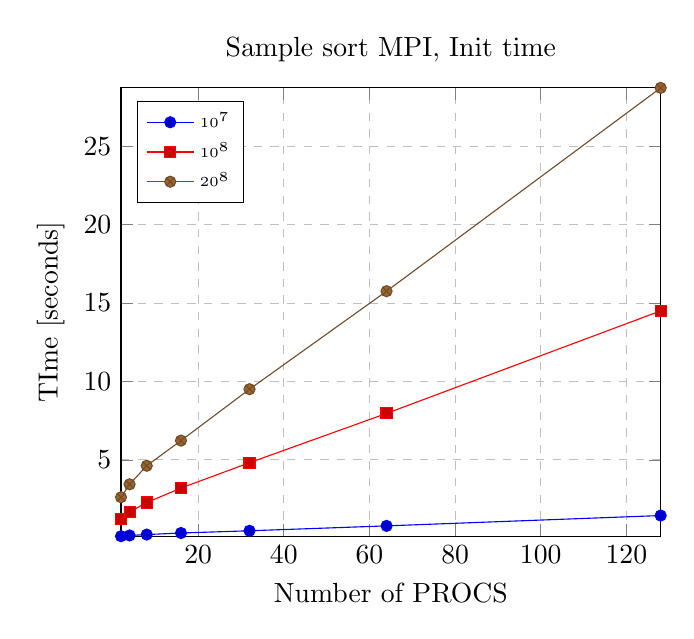
\begin{tikzpicture}
\begin{axis}[
title={Sample sort MPI, Init time},
xlabel={Number of PROCS},
ylabel={TIme [seconds]},
ymajorgrids=true,
xmajorgrids=true,
grid style=dashed,
enlargelimits=false,
scaled y ticks=false,
legend style={legend pos=north west, font=\fontsize{4}{5}\selectfont},
]

\addplot coordinates {
(2       , 0.138452  )
(4       , 0.185141  )
(8       , 0.242020  )
(16      , 0.341155  )
(32      , 0.483507  )
(64      , 0.795968  )
(128     , 1.455180  )
}; \addlegendentry{$10^7$}

\addplot coordinates {
(2       , 1.251224  )
(4       , 1.686172  )
(8       , 2.281364  )
(16      , 3.207226  )
(32      , 4.821805  )
(64      , 7.966258  )
(128     , 14.501871 )
}; \addlegendentry{$10^8$}

\addplot coordinates {
(2       , 2.621422  )
(4       , 3.446991  )
(8       , 4.629498  )
(16      , 6.232561  )
(32      , 9.509105  )
(64      , 15.756555 )
(128     , 28.718129 )
}; \addlegendentry{$20^8$}

\end{axis}
\end{tikzpicture}

\noindent Although it is not clear for me why this operation was the slowest performer,
especially on larger
number of procs, since it is always executed only by the host machine.
Initialization time was linearly increasing with number of participating
procs, i.e. only number of procs affected init performance but not the data set size.


\vspace{0.5cm}

Other intervals behaved as expected:

\begin{itemize}
\item Sort stage performance increase is log(n), where n is number of procs. 
\item Data send time decrease is log(n), where n is number of procs (more messages however
each message has smaller size).
\item File read time is minuscule compared to all other operations (about \%0.7 in average
for all cases).
\item Total IO (read data set + save results), is mostly affected by the save stage. Save
stage pattern is similar to the patter of Total Time, with the sweet spot being nporcs = 64.
This was expected since larger number of procs will have more data movements across network.
\end{itemize}

\begin{minipage}{0.52\textwidth}
\begin{centering}
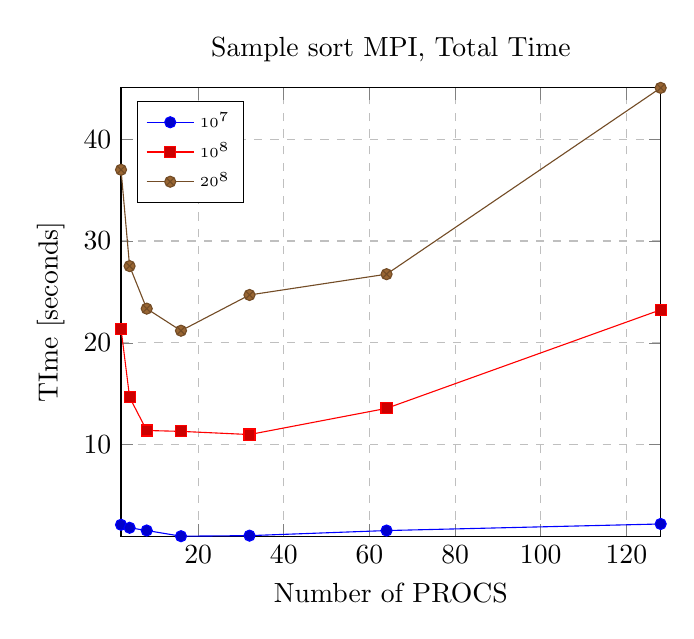
\begin{tikzpicture}
\begin{axis}[
title={Sample sort MPI, Total Time},
xlabel={Number of PROCS},
ylabel={TIme [seconds]},
ymajorgrids=true,
xmajorgrids=true,
grid style=dashed,
enlargelimits=false,
scaled y ticks=false,
legend style={legend pos=north west, font=\fontsize{4}{5}\selectfont},
]

\addplot coordinates { 
(2,2.148589)
(4,1.854079)
(8,1.585789)
(16,1.026434)
(32,1.081793)
(64,1.580246)
(128,2.226394)
}; \addlegendentry{$10^7$}
\addplot coordinates { 
(2,21.388325)
(4,14.662842)
(8,11.401545)
(16,11.315433)
(32,11.003947)
(64,13.574712)
(128,23.246394)
}; \addlegendentry{$10^8$}
\addplot coordinates { 
(2,36.989818)
(4,27.535513)
(8,23.360451)
(16,21.193418)
(32,24.702475)
(64,26.741631)
(128,45.027526)
}; \addlegendentry{$20^8$}
\end{axis}
\end{tikzpicture}
\end{centering}
\end{minipage}%
\begin{minipage}{0.52\textwidth}
\begin{centering}
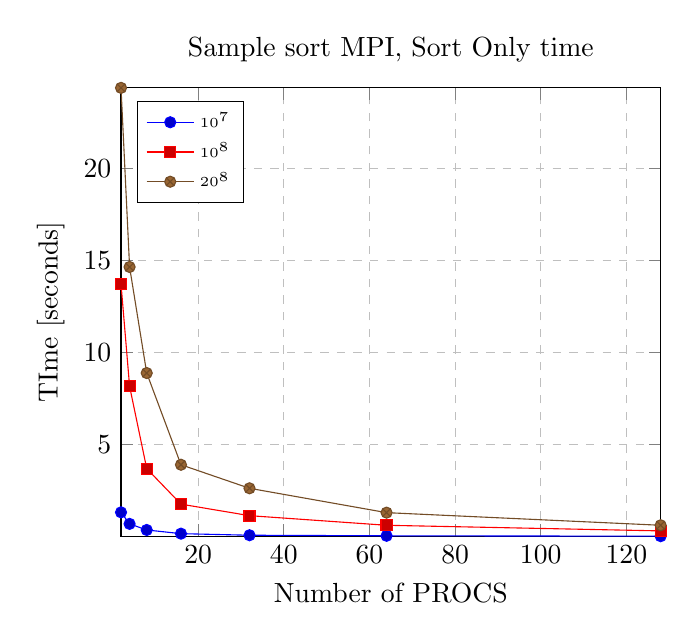
\begin{tikzpicture}
\begin{axis}[
title={Sample sort MPI, Sort Only time},
xlabel={Number of PROCS},
ylabel={TIme [seconds]},
ymajorgrids=true,
xmajorgrids=true,
grid style=dashed,
enlargelimits=false,
scaled y ticks=false,
legend style={legend pos=north west, font=\fontsize{4}{5}\selectfont},
]

\addplot coordinates {
(2,1.329322)
(4,0.703482)
(8,0.372035)
(16,0.172070)
(32,0.086430)
(64,0.055387)
(128,0.034200)
}; \addlegendentry{$10^7$}

\addplot coordinates {
(2,13.715294)
(4,8.170872)
(8,3.704629)
(16,1.774006)
(32,1.149074)
(64,0.626844)
(128,0.322027)
}; \addlegendentry{$10^8$}

\addplot coordinates {
(2,24.375176)
(4,14.650789)
(8,8.892560)
(16,3.913000)
(32,2.635067)
(64,1.312693)
(128,0.627599)
}; \addlegendentry{$20^8$}

\end{axis}
\end{tikzpicture}
\end{centering}
\end{minipage}%


\begin{minipage}{0.52\textwidth}
\begin{centering}
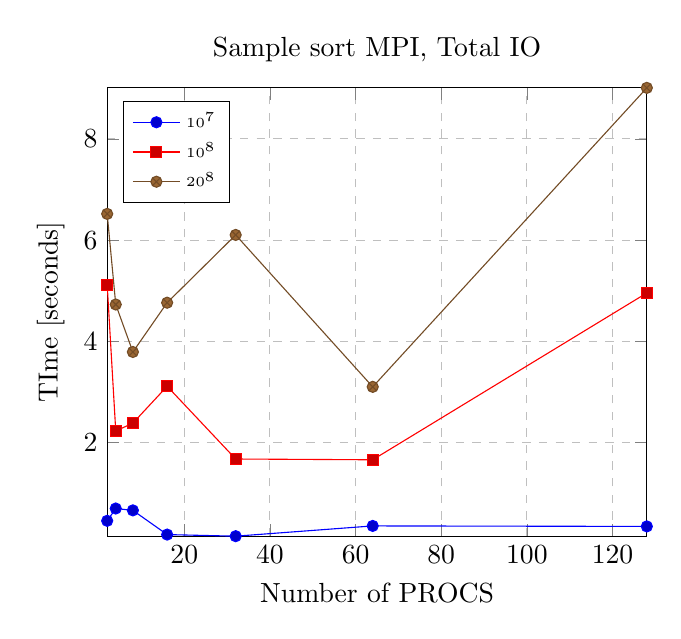
\begin{tikzpicture}
\begin{axis}[
title={Sample sort MPI, Total IO},
xlabel={Number of PROCS},
ylabel={TIme [seconds]},
ymajorgrids=true,
xmajorgrids=true,
grid style=dashed,
enlargelimits=false,
scaled y ticks=false,
legend style={legend pos=north west, font=\fontsize{4}{5}\selectfont},
]
\addplot coordinates {
(2,0.457513)
(4,0.700616)
(8,0.663785)
(16,0.185904)
(32,0.154169)
(64,0.356824)
(128,0.347138)
}; \addlegendentry{$10^7$}
\addplot coordinates {
(2,5.119837)
(4,2.230569)
(8,2.386517)
(16,3.114079)
(32,1.677889)
(64,1.662745)
(128,4.956577)
}; \addlegendentry{$10^8$}
\addplot coordinates {
(2,6.517857)
(4,4.728756)
(8,3.791264)
(16,4.764139)
(32,6.102151)
(64,3.102582)
(128,9.005717)
}; \addlegendentry{$20^8$}

\end{axis}
\end{tikzpicture}
\end{centering}
\end{minipage}%
\begin{minipage}{0.52\textwidth}
\begin{centering}
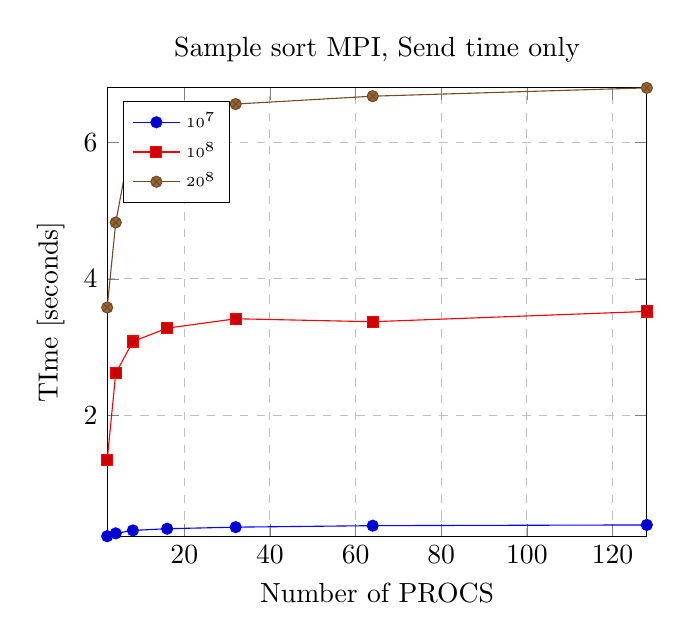
\begin{tikzpicture}
\begin{axis}[
title={Sample sort MPI, Send time only},
xlabel={Number of PROCS},
ylabel={TIme [seconds]},
ymajorgrids=true,
xmajorgrids=true,
grid style=dashed,
enlargelimits=false,
scaled y ticks=false,
legend style={legend pos=north west, font=\fontsize{4}{5}\selectfont},
]

\addplot coordinates {
(2,0.230972)
(4,0.272491)
(8,0.315651)
(16,0.340391)
(32,0.363428)
(64,0.385250)
(128,0.395844)
}; \addlegendentry{$10^7$}
\addplot coordinates {
(2,1.346666)
(4,2.618578)
(8,3.082428)
(16,3.277671)
(32,3.415177)
(64,3.371693)
(128,3.522364)
}; \addlegendentry{$10^8$}
\addplot coordinates {
(2,3.579794)
(4,4.824926)
(8,6.164339)
(16,6.393795)
(32,6.559370)
(64,6.674599)
(128,6.796331)
}; \addlegendentry{$20^8$}
\end{axis}
\end{tikzpicture}
\end{centering}
\end{minipage}

\vspace{0.4cm}

Following bar charts show normalized (to total time = \%100) distribution of different
program intervals (in percent), 
each chart represents different number of procs, in the order of $2, 4, 8, 16,32, 64, 128$


\vspace{0.4cm}

\begin{minipage}{0.52\textwidth}
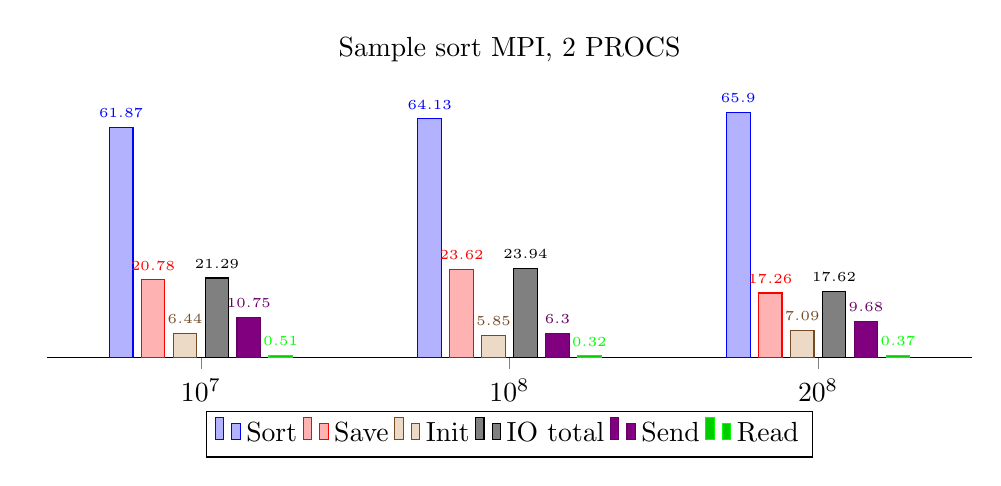
\begin{tikzpicture}
%\begin{semilogxaxis}
%\begin{loglogaxis}
\begin{axis} [ 
title={Sample sort MPI, 2 PROCS},
compat=newest,
legend style={at={(0.5,-0.20)},anchor=north,legend columns=0},
xtick={6,10,14},
%symbolic x coords={1982, 1990, 1999, 2006},
xticklabels={
    {$10^7$},
    {$10^8$},
    {$20^8$}},
nodes near coords,
every node near coord/.append style={font=\tiny},
axis lines*=left,
y axis line style={opacity=0},
yticklabels={\empty},
ytick style={draw=none},
ymin=0.0,
xmax=16,
xmin=4.0,
% ylabel={Time [seconds]},
ybar=3pt,
% ymajorgrids=true,
% xmajorgrids=true,
% grid style=dashed,
% enlargelimits=0.75,
height=5cm, 
bar width=0.3cm,
%bar shift=0pt,
width=1.1\textwidth, 
        ]
    \addplot+[ybar] plot coordinates { (6,61.8695339127)  (10,64.1251430395) (14,65.8969881928)  }; %Sort
    \addplot+[ybar] plot coordinates { (6,20.7793114458)  (10,23.6224903072) (14,17.255643161)   }; %Save
    \addplot+[ybar] plot coordinates { (6,6.44385687537)  (10,5.85003266969) (14,7.08687455559)  }; %Init
    \addplot+[ybar] plot coordinates { (6,21.2936489948)  (10,23.9375313401) (14,17.62067875)    };  %IO Total
    \addplot+[ybar] plot coordinates { (6,10.7499386807)  (10,6.29626677171) (14,9.67778213994)  };  %Send
    \addplot+[ybar] plot coordinates { (6,0.514337548968)  (10,0.3150410329) (14,0.365035588983) }; %Read
\legend{Sort, Save, Init, IO total,  Send, Read}
%\end{loglogaxis}
%\end{semilogxaxis}
\end{axis}
\end{tikzpicture}
\end{minipage}%
\begin{minipage}{0.52\textwidth}
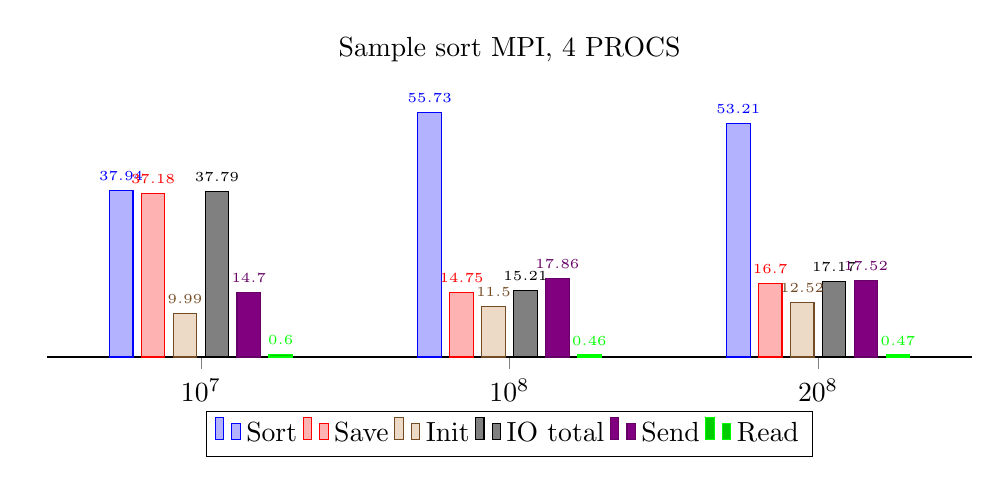
\begin{tikzpicture}
\begin{axis} [ 
compat=newest,
title={Sample sort MPI, 4 PROCS},
legend style={at={(0.5,-0.20)},anchor=north,legend columns=0},
xtick={6,10,14},
%symbolic x coords={1982, 1990, 1999, 2006},
xticklabels={
    {$10^7$},
    {$10^8$},
    {$20^8$}},
nodes near coords,
every node near coord/.append style={font=\tiny},
axis lines*=left,
y axis line style={opacity=0},
yticklabels={\empty},
ytick style={draw=none},
ymin=0.0,
xmax=16,
xmin=4.0,
% ylabel={Time [seconds]},
ybar=3pt,
% ymajorgrids=true,
% xmajorgrids=true,
% grid style=dashed,
% enlargelimits=0.75,
height=5cm, 
bar width=0.3cm,
%bar shift=0pt,
width=1.1\textwidth, 
        ]

    \addplot+[ybar] plot coordinates { (6,37.9423961978)  (10,55.7250224752) (14,53.2068859585)    };   %Sort
    \addplot+[ybar] plot coordinates { (6,37.1845536247)  (10,14.7488324569) (14,16.7023399927)    };   %Save
    \addplot+[ybar] plot coordinates { (6,9.98560471264)  (10,11.4996260616) (14,12.5183467619)    };   %Init
    \addplot+[ybar] plot coordinates { (6,37.7878181027)  (10,15.2123919769) (14,17.1732990774)    }; %IO Total
    \addplot+[ybar] plot coordinates { (6,14.6968387)  (10,17.8585979444) (14,17.5225571428)       }; %Send
    \addplot+[ybar] plot coordinates { (6,0.603264477943)  (10,0.463559520044) (14,0.470959084728) };   %Read

\legend{Sort, Save, Init, IO total,  Send, Read}
%\end{loglogaxis}
%\end{semilogxaxis}
\end{axis}
\end{tikzpicture}
\end{minipage}%

\vspace{0.3cm}
Two and four spend most of the time $\approx \%60$ in sorting.
\vspace{0.3cm}

\begin{minipage}{0.52\textwidth}
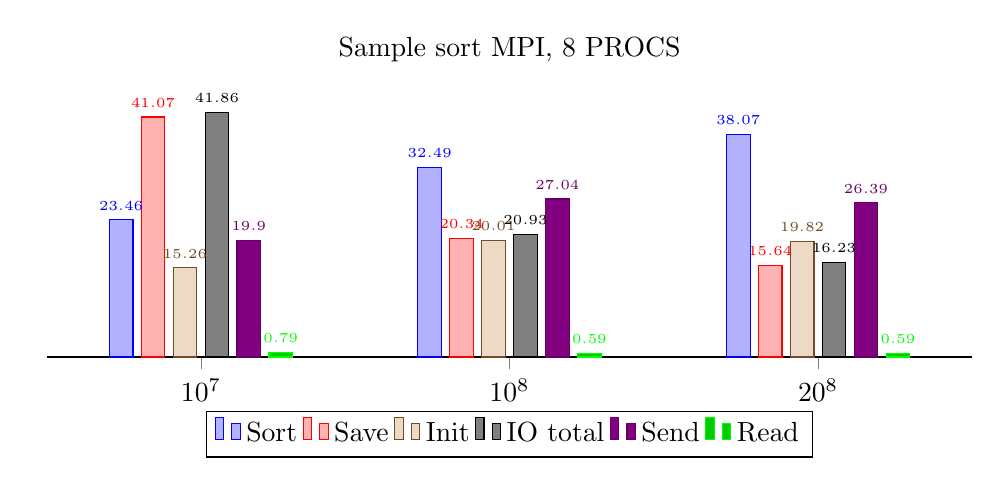
\begin{tikzpicture}
%\begin{semilogxaxis}
%\begin{loglogaxis}
\begin{axis} [ 
compat=newest,
title={Sample sort MPI, 8 PROCS},
legend style={at={(0.5,-0.20)},anchor=north,legend columns=0},
xtick={6,10,14},
%symbolic x coords={1982, 1990, 1999, 2006},
xticklabels={
    {$10^7$},
    {$10^8$},
    {$20^8$}},
nodes near coords,
every node near coord/.append style={font=\tiny},
axis lines*=left,
y axis line style={opacity=0},
yticklabels={\empty},
ytick style={draw=none},
ymin=0.0,
xmax=16,
xmin=4.0,
% ylabel={Time [seconds]},
ybar=3pt,
% ymajorgrids=true,
% xmajorgrids=true,
% grid style=dashed,
% enlargelimits=0.75,
height=5cm, 
bar width=0.3cm,
%bar shift=0pt,
width=1.1\textwidth, 
        ]
    \addplot+[ybar] plot coordinates { (6,23.4605612727)  (10,32.4923420466) (14,38.0667308178)    };     %Sort
    \addplot+[ybar] plot coordinates { (6,41.0671911585)  (10,20.3413923288) (14,15.6438888958)    };     %Save
    \addplot+[ybar] plot coordinates { (6,15.2618034303)  (10,20.0092531319) (14,19.8176738968)    };     %Init
    \addplot+[ybar] plot coordinates { (6,41.8583430709)  (10,20.9315228769) (14,16.2294126941)    };  %IO Total
    \addplot+[ybar] plot coordinates { (6,19.9049810536)  (10,27.0351781272) (14,26.3879280413)    };  %Send
    \addplot+[ybar] plot coordinates { (6,0.791151912392)  (10,0.590130548097) (14,0.585523798321) };     %Read
\legend{Sort, Save, Init, IO total,  Send, Read}
%\end{loglogaxis}
%\end{semilogxaxis}
\end{axis}
\end{tikzpicture}
\end{minipage}%
\begin{minipage}{0.52\textwidth}
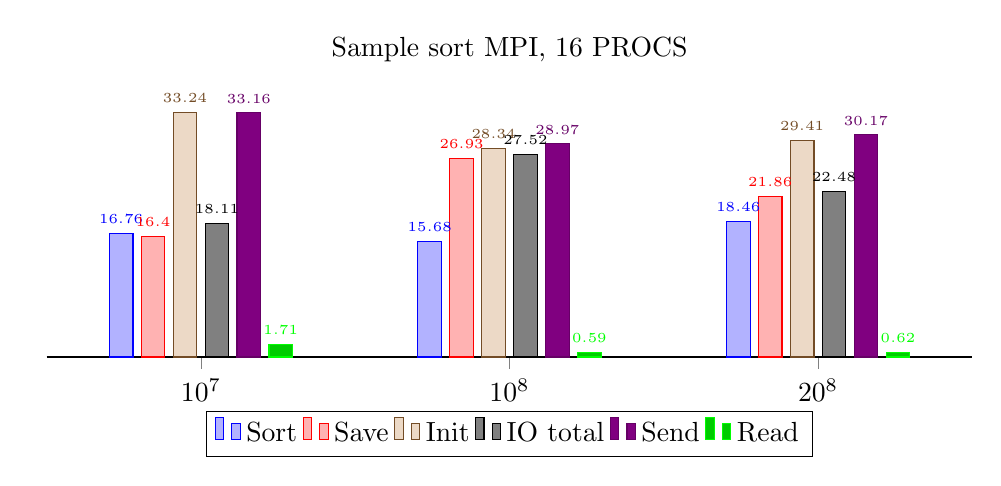
\begin{tikzpicture}
\begin{axis} [ 
compat=newest,
title={Sample sort MPI, 16 PROCS},
legend style={at={(0.5,-0.20)},anchor=north,legend columns=0},
xtick={6,10,14},
%symbolic x coords={1982, 1990, 1999, 2006},
xticklabels={
    {$10^7$},
    {$10^8$},
    {$20^8$}},
nodes near coords,
every node near coord/.append style={font=\tiny},
axis lines*=left,
y axis line style={opacity=0},
yticklabels={\empty},
ytick style={draw=none},
ymin=0.0,
xmax=16,
xmin=4.0,
% ylabel={Time [seconds]},
ybar=3pt,
% ymajorgrids=true,
% xmajorgrids=true,
% grid style=dashed,
% enlargelimits=0.75,
height=5cm, 
bar width=0.3cm,
%bar shift=0pt,
width=1.1\textwidth, 
        ]
    \addplot+[ybar] plot coordinates { (6,16.7638640185)  (10,15.6777562114) (14,18.4632794955)   };     %Sort
    \addplot+[ybar] plot coordinates { (6,16.4046592377)  (10,26.931245141) (14,21.8592300685)    };     %Save
    \addplot+[ybar] plot coordinates { (6,33.2369153789)  (10,28.3438203381) (14,29.4080029941)   };     %Init
    \addplot+[ybar] plot coordinates { (6,18.1116369879)  (10,27.520634871) (14,22.4793329703)    };  %IO Total
    \addplot+[ybar] plot coordinates { (6,33.1624829263)  (10,28.9663771594) (14,30.1687769288)   };  %Send
    \addplot+[ybar] plot coordinates { (6,1.70697775015)  (10,0.589389729938) (14,0.620102901759) };     %Read
\legend{Sort, Save, Init, IO total,  Send, Read}
%\end{loglogaxis}
%\end{semilogxaxis}
\end{axis}
\end{tikzpicture}
\end{minipage}
8 and 16 (fastest ones) have about equal load distribution.


\pagebreak

All the rest spend most of the time in initialization stage\\
\vspace{1cm}

\begin{minipage}{0.52\textwidth}
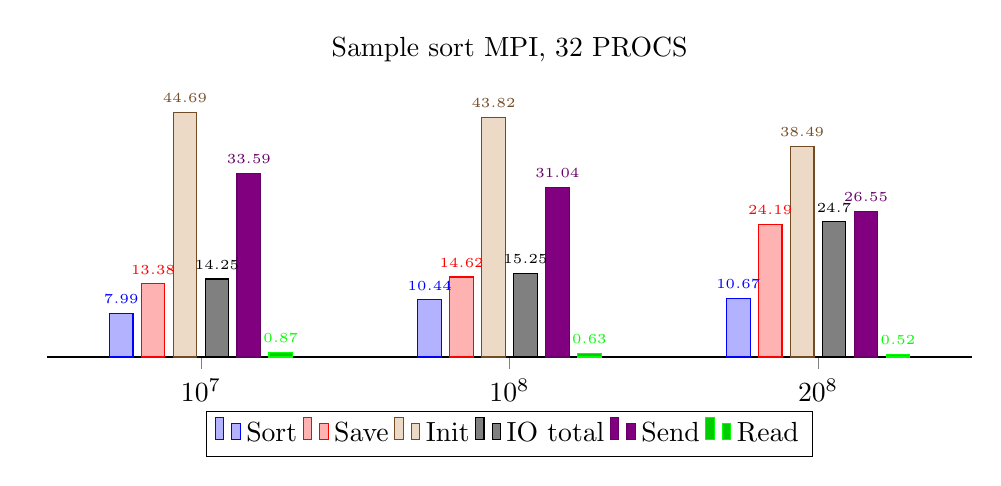
\begin{tikzpicture}
%\begin{semilogxaxis}
%\begin{loglogaxis}
\begin{axis} [ 
compat=newest,
title={Sample sort MPI, 32 PROCS},
legend style={at={(0.5,-0.20)},anchor=north,legend columns=0},
xtick={6,10,14},
%symbolic x coords={1982, 1990, 1999, 2006},
xticklabels={
    {$10^7$},
    {$10^8$},
    {$20^8$}},
nodes near coords,
every node near coord/.append style={font=\tiny},
axis lines*=left,
y axis line style={opacity=0},
yticklabels={\empty},
ytick style={draw=none},
ymin=0.0,
xmax=16,
xmin=4.0,
% ylabel={Time [seconds]},
ybar=3pt,
% ymajorgrids=true,
% xmajorgrids=true,
% grid style=dashed,
% enlargelimits=0.75,
height=5cm, 
bar width=0.3cm,
%bar shift=0pt,
width=1.1\textwidth, 
        ]
    \addplot+[ybar] plot coordinates { (6,7.98951370549)  (10,10.4423803568) (14,10.6672185682)    };     %Sort
    \addplot+[ybar] plot coordinates { (6,13.3787147818)  (10,14.6217352737) (14,24.1856453655)    };     %Save
    \addplot+[ybar] plot coordinates { (6,44.6949647483)  (10,43.8188679026) (14,38.4945435629)    };     %Init
    \addplot+[ybar] plot coordinates { (6,14.2512476971)  (10,15.2480650806) (14,24.7025895179)    };  %IO Total
    \addplot+[ybar] plot coordinates { (6,33.5949668744)  (10,31.0359273813) (14,26.5534931216)    };  %Send
    \addplot+[ybar] plot coordinates { (6,0.872532915262)  (10,0.626329806932) (14,0.516944152357) };     %Read
\legend{Sort, Save, Init, IO total,  Send, Read}
\end{axis}
\end{tikzpicture}
\end{minipage}%
\begin{minipage}{0.52\textwidth}
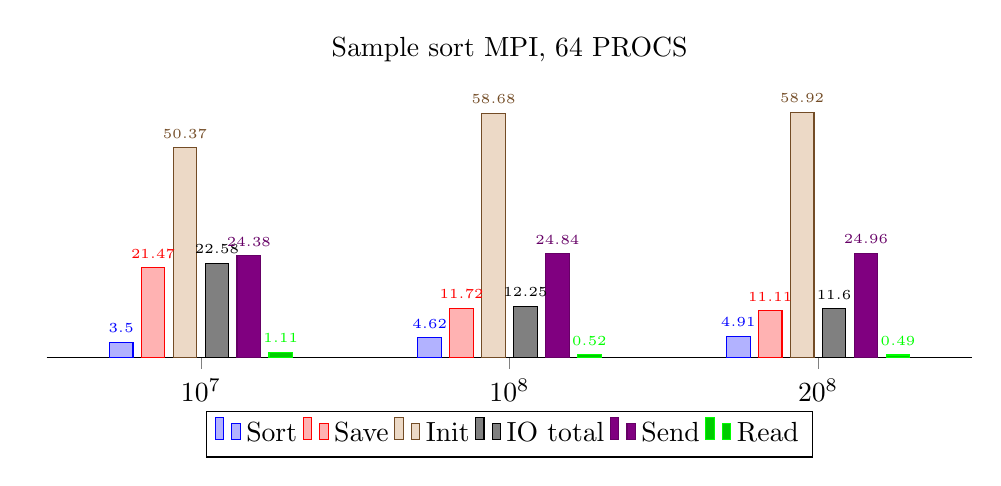
\begin{tikzpicture}
\begin{axis} [ 
compat=newest,
title={Sample sort MPI, 64 PROCS},
legend style={at={(0.5,-0.20)},anchor=north,legend columns=0},
xtick={6,10,14},
xticklabels={
    {$10^7$},
    {$10^8$},
    {$20^8$}},
nodes near coords,
every node near coord/.append style={font=\tiny},
axis lines*=left,
y axis line style={opacity=0},
yticklabels={\empty},
ytick style={draw=none},
ymin=0.0,
xmax=16,
xmin=4.0,
ybar=3pt,
% enlargelimits=0.75,
height=5cm, 
bar width=0.3cm,
%bar shift=0pt,
width=1.1\textwidth, 
        ]
    \addplot+[ybar] plot coordinates { (6,3.50496062006)  (10,4.6177333265) (14,4.90879931744)   };     %Sort
    \addplot+[ybar] plot coordinates { (6,21.4671639732)  (10,11.7248822664) (14,11.1135405316)  };     %Save
    \addplot+[ybar] plot coordinates { (6,50.3698791201)  (10,58.6845452043) (14,58.9214434976)  };     %Init
    \addplot+[ybar] plot coordinates { (6,22.5802818042)  (10,12.248841817) (14,11.6020672038)   };  %IO Total
    \addplot+[ybar] plot coordinates { (6,24.3791156567)  (10,24.8380444462) (14,24.9595808124)  };  %Send
    \addplot+[ybar] plot coordinates { (6,1.11311783102)  (10,0.52395955067) (14,0.488526672139) };     %Read
\legend{Sort, Save, Init, IO total,  Send, Read}
\end{axis}
\end{tikzpicture}
\end{minipage}%

\vspace{1.1cm}

\begin{minipage}{0.52\textwidth}
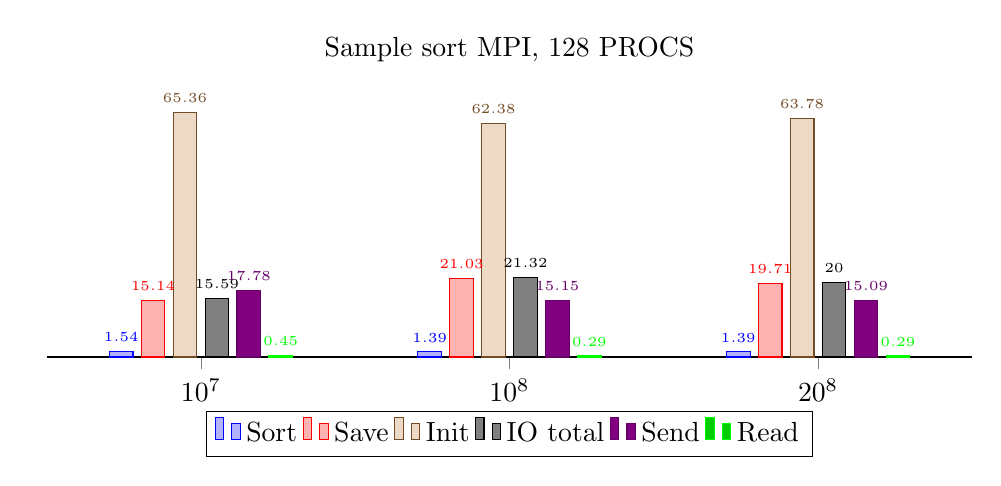
\begin{tikzpicture}
\begin{axis} [ 
compat=newest,
title={Sample sort MPI, 128 PROCS},
legend style={at={(0.5,-0.20)},anchor=north,legend columns=0},
xtick={6,10,14},
xticklabels={
    {$10^7$},
    {$10^8$},
    {$20^8$}},
nodes near coords,
every node near coord/.append style={font=\tiny},
axis lines*=left,
y axis line style={opacity=0},
yticklabels={\empty},
ytick style={draw=none},
ymin=0.0,
xmax=16,
xmin=4.0,
ybar=3pt,
% enlargelimits=0.75,
height=5cm, 
bar width=0.3cm,
%bar shift=0pt,
width=1.1\textwidth, 
        ]
    \addplot+[ybar] plot coordinates { (6,1.53611624897)  (10,1.38527721762) (14,1.39381186521)    };     %Sort
    \addplot+[ybar] plot coordinates { (6,15.1370332475)  (10,21.0321824538) (14,19.7059860673)    };     %Save
    \addplot+[ybar] plot coordinates { (6,65.3603989231)  (10,62.3833141605) (14,63.7790515073)    };     %Init
    \addplot+[ybar] plot coordinates { (6,15.5919392524)  (10,21.3219177133) (14,20.0004703789)    };  %IO Total
    \addplot+[ybar] plot coordinates { (6,17.7796023525)  (10,15.1523027615) (14,15.0937251138)    };  %Send
    \addplot+[ybar] plot coordinates { (6,0.454906004957)  (10,0.289735259585) (14,0.294484311663) };     %Read
\legend{Sort, Save, Init, IO total,  Send, Read}
\end{axis}
\end{tikzpicture}
\end{minipage}%

\end{document}
